%------------------------------------------------------------------------------
% CV in Latex
% Author : Charles Rambo
% Based off of: https://github.com/sb2nov/resume and Jake's Resume on Overleaf
% Most recently updated version may be found at https://github.com/fizixmastr 
% License : MIT
%------------------------------------------------------------------------------

\documentclass[A4,11pt]{article}
\usepackage{latexsym}
\usepackage[empty]{fullpage}
\usepackage{titlesec}
\usepackage{marvosym}
\usepackage[usenames,dvipsnames]{color}
\usepackage{verbatim}
\usepackage{enumitem}
\usepackage[hidelinks]{hyperref}
\usepackage[english]{babel}
\usepackage{tabularx}
\usepackage{tikz}
\input{glyphtounicode}

% \usepackage[latin1]{inputenc}
\usepackage[english]{babel}
\usepackage[T1]{fontenc}
\usepackage{fontawesome}
\usepackage{graphicx,wrapfig}
\usepackage{url}


% serif
 \usepackage{palatino}
% \usepackage{times} %This is the default as well
% \usepackage{charter}

% sans-serif
% \usepackage{helvet}
% \usepackage[sfdefault]{noto-sans}
% \usepackage[default]{sourcesanspro}

%-----PAGE SETUP---------------------------------------------------------------

% Adjust margins
\addtolength{\oddsidemargin}{-1cm}
\addtolength{\evensidemargin}{-1cm}
\addtolength{\textwidth}{2cm}
\addtolength{\topmargin}{-1cm}
\addtolength{\textheight}{2cm}

% Margins for US Letter size
%\addtolength{\oddsidemargin}{-0.5in}
%\addtolength{\evensidemargin}{-0.5in}
%\addtolength{\textwidth}{1in}
%\addtolength{\topmargin}{-.5in}
%\addtolength{\textheight}{1.0in}

\urlstyle{same}

\raggedbottom
\raggedright
\setlength{\tabcolsep}{0cm}

% Sections formatting
\titleformat{\section}{
  \vspace{-4pt}\scshape\raggedright\large
}{}{0em}{}[\color{black}\titlerule \vspace{-5pt}]

% Ensure that .pdf is machine readable/ATS parsable
\pdfgentounicode=1

%-----CUSTOM COMMANDS FOR FORMATTING SECTIONS----------------------------------
\newcommand{\CVItem}[1]{
  \item\small{
    {#1 \vspace{-2pt}}
  }
}

\newcommand{\CVSubheading}[4]{
  \vspace{-2pt}\item
    \begin{tabular*}{0.97\textwidth}[t]{l@{\extracolsep{\fill}}r}
      \textbf{#1} & #2 \\
      \small#3 & \small #4 \\
    \end{tabular*}\vspace{-7pt}
}

\newcommand{\CVSubSubheading}[2]{
    \item
    \begin{tabular*}{0.97\textwidth}{l@{\extracolsep{\fill}}r}
      \text{\small#1} & \text{\small #2} \\
    \end{tabular*}\vspace{-7pt}
}

\newcommand{\CVSubItem}[1]{\CVItem{#1}\vspace{-4pt}}

\renewcommand\labelitemii{$\vcenter{\hbox{\tiny$\bullet$}}$}

\newcommand{\CVSubHeadingListStart}{\begin{itemize}[leftmargin=0.5cm, label={}]}
% \newcommand{\resumeSubHeadingListStart}{\begin{itemize}[leftmargin=0.15in, label={}]} % Uncomment for US
\newcommand{\CVSubHeadingListEnd}{\end{itemize}}
\newcommand{\CVItemListStart}{\begin{itemize}}
\newcommand{\CVItemListEnd}{\end{itemize}\vspace{-5pt}}

%------------------------------------------------------------------------------
% CV STARTS HERE  %
%------------------------------------------------------------------------------
\begin{document}

%-----HEADING------------------------------------------------------------------
\begin{comment}
In Europe it is common to include a picture of ones self in the CV. Select
which heading appropriate for the document you are creating.
\end{comment}

\begin{minipage}[c]{0.05\textwidth}
\-\
\end{minipage}
\begin{minipage}[c]{0.2\textwidth}
% \begin{tikzpicture}
%     \clip (0,0) circle (1.75cm);
%     \node at (0,-.7) {\includegraphics[scale=0.2]{bright_photo_image.jpg}}; 
%     % if necessary the picture may be moved by changing the at (coordinates)
%     % width defines the 'zoom' of the picture
% \end{tikzpicture}
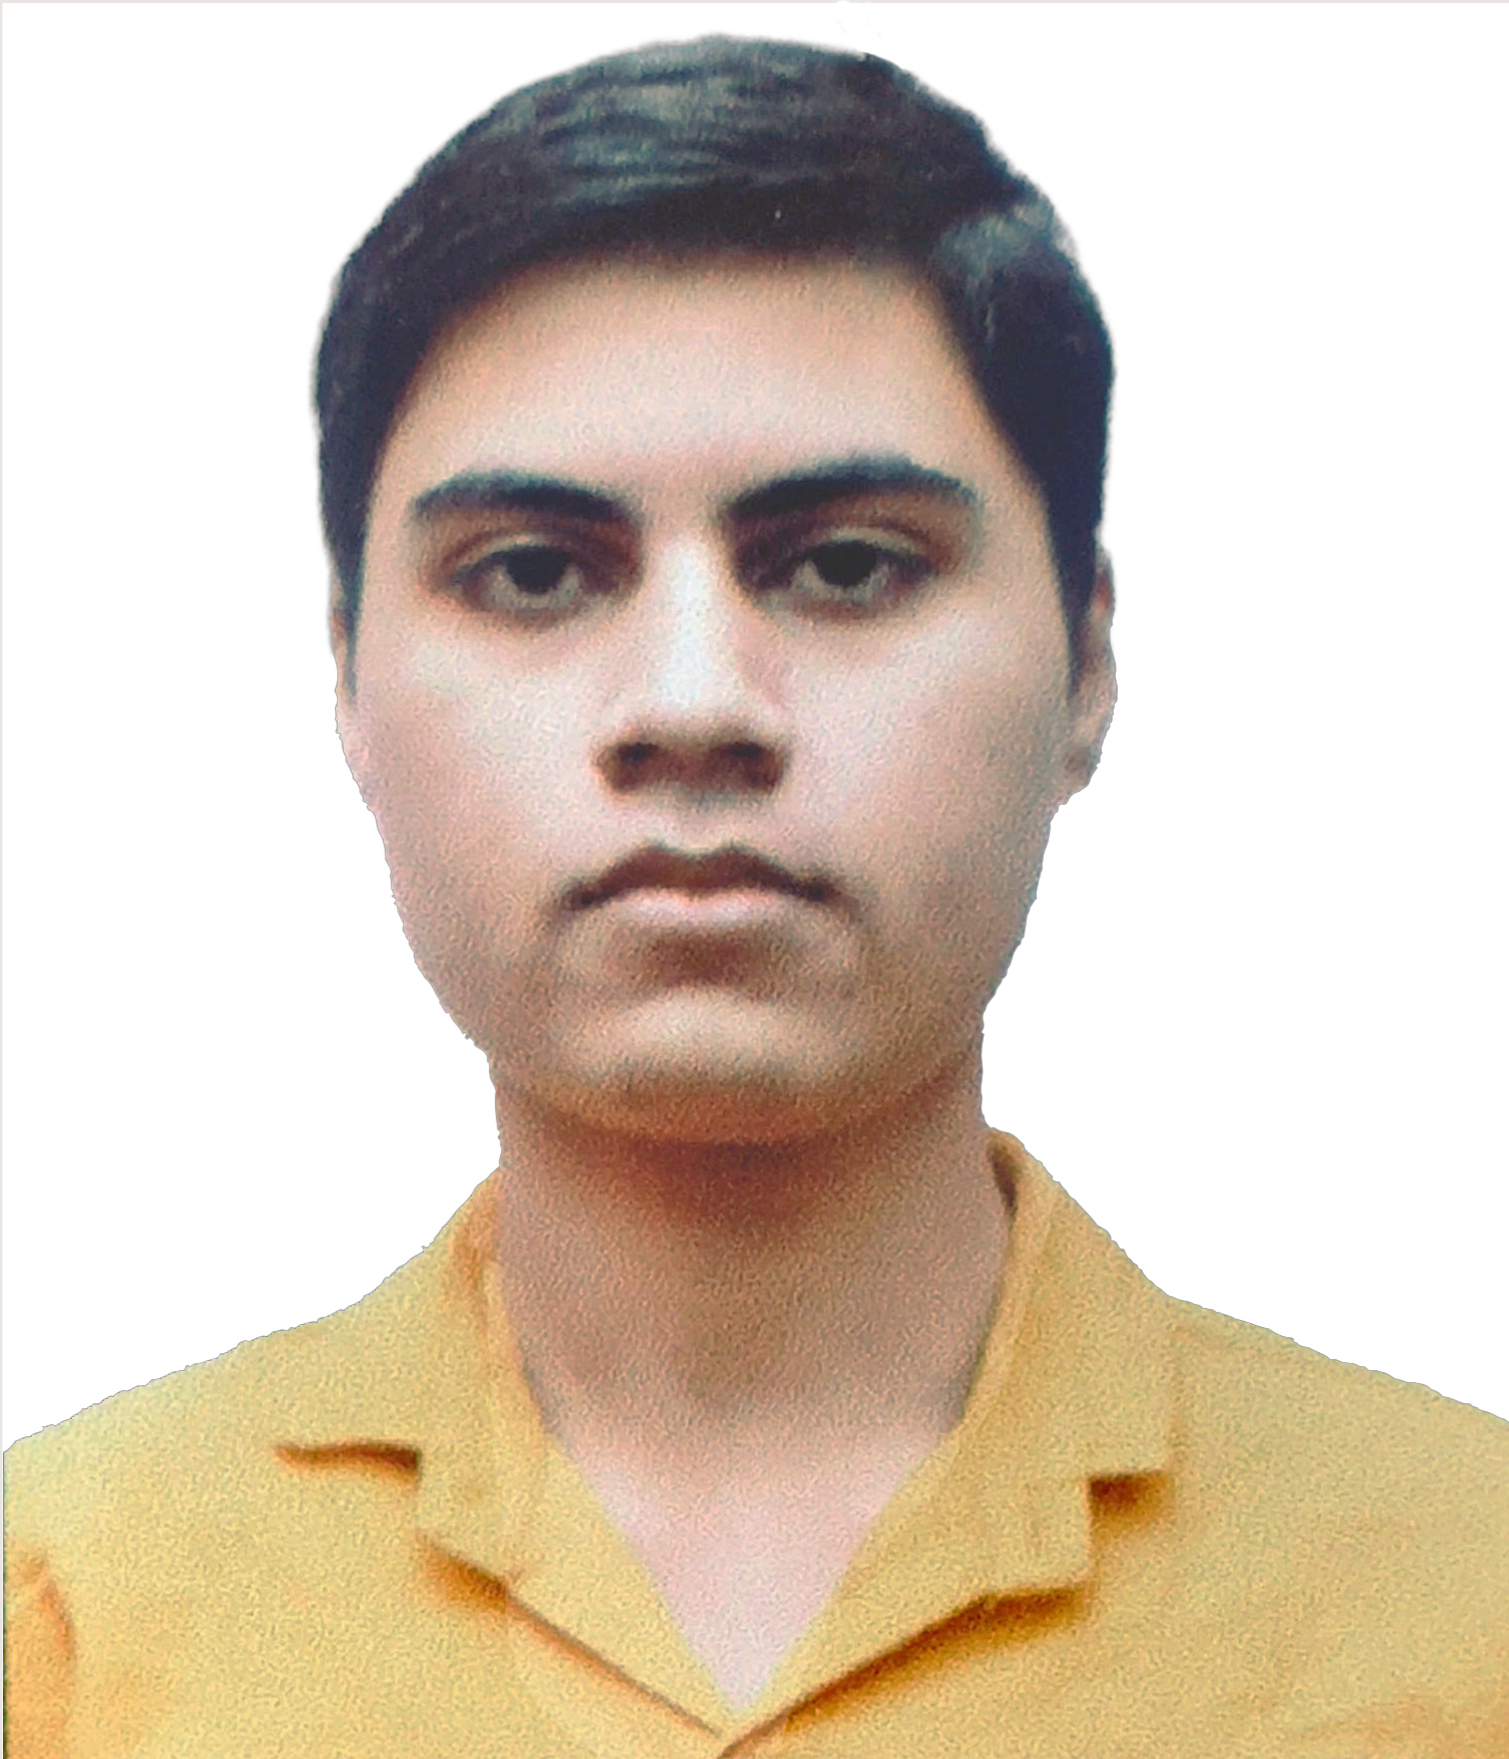
\includegraphics[scale=0.25]{components/portrait.jpg}
\hfill\vline\hfill
\end{minipage}
\begin{minipage}[c]{0.4\textwidth}
    \textbf{\Huge \scshape{\hspace{3pt}Rohit Khare}} \\ \vspace{1pt} \\
    % \scshape sets small capital letters, remove if desired
    \hspace*{3pt}\small{\faPhone\hspace{2pt}+91 8770749004} \\ 
    \href{mailto:rohit97528@gmail.com}{\hspace{3pt}\faEnvelope\underline{ rohit97528@gmail.com}} \\
    % Be sure to use a professional *personal* email address
    \href{https://github.com/notr0hit}{\hspace{3pt}\faGithub \underline{ github.com/notr0hit}} \\
    % \href{https://www.linkedin.com/in/charles-rambo/}{\underline{linkedin.com/in/charles-rambo}} \\
     \href{https://codeforces.com/profile/not_rohit}{\hspace{3pt}
\includegraphics[scale=0.008]{components/codeforces.jpg} \underline{codeforces.com/not\_rohit}} 
    
    \href{https://www.codechef.com/users/not_rohit}{\hspace{3pt}
\includegraphics[scale=0.008]{components/codechef.jpg} \underline{codechef.com/not\_rohit}} \\
    % you should adjust you linked in profile name to be professional and recognizable
    
\end{minipage}

\vspace*{2pt}

% Without picture
%\begin{center}
%    \textbf{\Huge \scshape Charles Rambo} \\ \vspace{1pt} %\scshape sets small capital letters, remove if desired
%    \small +1 123-456-7890 $|$ 
%    \href{mailto:you@provider.com}{\underline{you@provider.com}} $|$\\
%    % Be sure to use a professional *personal* email address
%    \href{https://linkedin.com/in/your-name-here}{\underline{linkedin.com/in/charles-rambo}} $|$
%    % you should adjust you linked in profile name to be professional and recognizable
%    \href{https://github.com/fizixmastr}{\underline{github.com/fizixmastr}}
%\end{center}

%-----EDUCATION----------------------------------------------------------------
\section{education}
  \CVSubHeadingListStart
%    \CVSubheading % Example
%      {Degree Achieved}{Years of Study}
%      {Institution of Study}{Where it is located}
    \CVSubheading
      {{Maulana Azad National Institute Of Technology, Bhopal}}{\emph{December 2020 - Present}}
      {B.Tech in Computer Science And Engineering}{CGPA: 8.58}
    \CVSubheading
      {{Sanskar Public School, Gwalior}}{\emph{2019-2020}}
      {12th Grade}{Overall Percentage: 82.6}
    \CVSubheading
      {{Pragati Vidya Peeth, Gwalior}}{\emph{2017-2018}}
      {10th Grade}{Overall Percentage: 87.4} \\
  \CVSubHeadingListEnd

\vspace*{3pt}
% %-----PROJECTS----------------------------------------------------
% \begin{comment}
% Ideally the title of the work should speak for what it is. However if you feel
% like you should explain more about why the project is applicable to this job,
% use item list as is shown in the work experience section.
% \end{comment}

\section{technical skills}
 \begin{itemize}[leftmargin=0.5cm, label={}]
    \small{\item{
     \textbf{Programming Languages}{: C, C++, Python, Java} \\
     \textbf{Tools}{: Vim, Git}
    }}
 \end{itemize}

\vspace{1pt}

\section{projects}
  \CVSubHeadingListStart
%    \CVSubheading
%      {Title of Work}{When it was done}
%      {Institution you worked with}{unused}
    \CVSubheading
      {\href{https://github.com/notr0hit/website-summarizer/tree/main}{\underline{Website Summarizer}}}{}
      {A GUI based application written in Python, creates summary of website's text from its URL address. \vspace{3pt}}{}
      
    \CVSubheading
      {\href{https://github.com/notr0hit/twitch-chat-json-to-srt}{\underline{Twitch Chat Subtitle}}}{}
      {Python script which Shows Twitch chat messages as subtitles when watching \href{https://www.twitch.tv}{\underline{Twitch}} Videos in Video Player.\\
      Queue data structure was used to implement the algorithm for this script. \vspace{3pt}}{} 
      
      \CVSubheading
      {\href{https://github.com/notr0hit/wordle-solver-bot}{\underline{Wordle Solver}}}{}
      {C++ Application which solves the famous game \href{https://www.nytimes.com/games/wordle/index.html}{\underline{Wordle}} {(by New York Times).}}{}
  \CVSubHeadingListEnd 

\vspace*{3pt}

\section{achievements}
  \CVSubHeadingListStart
%    \CVSubheading
%      {Title of Work}{When it was done}
%      {Institution you worked with}{unused}
    \CVSubheading
      {Google Kickstart Round G}{\emph{October 2021}}
      {Achieved Rank 1711}{}
  
  \CVSubheading
    {Codeforces Educational Round 118}{\emph{December 2021}}      
    {Achieved Rank 2674}{} \\
  \CVSubHeadingListEnd

\vspace*{3pt}

\section{skills}
 \begin{itemize}[leftmargin=0.5cm, label={}]
    \small{\item{
     \textbf{Languages}{: English, Hindi (Native)} \\
    }}
 \end{itemize}
 
 \vspace*{1pt}

\section{hobbies and interests}
     \small{ \hspace*{11pt}
     Competitive Programming, Chess, Open Source Software, Problem Solving, Finance
     }

\end{document}